\section{Software Processes}

\subsection{Scrum Practices}

The project is being organized using ideas from Scrum, especially through iterative work, prioritization of tasks,
and the use of user stories.
The GitHub project board functions as a shared place for tasks and progress, and it helps the team keep track of ongoing work.

Sprint planning has been used to determine which user stories and tasks should be worked on in the current period.
One of the most important lessons so far is that Scrum practices only work when coordination is taken seriously.
If communication is weak, development becomes fragmented and some team members may end up waiting for others.

Because this is a student project, scheduling can also be difficult.
This makes it even more important to have visible tasks, frequent communication, and a shared understanding of current priorities.

\subsection{XP Practices}

The project also applies several ideas from Extreme Programming(XP).
These include continuous integration, automated testing, pair programming, and an emphasis on incremental development.
Not all XP practices are equally developed at this stage, but several are already visible in our workflow.


Continuous integration, described earlier, supports the XP principle of frequent integration
and early detection of errors.
In our project, this reduced integration problems and improved confidence when merging changes,
especially when multiple team members were working in parallel.

Testing is present through JUnit, although the testing framework is still expected to become more complete later in the project.
Similarly, practices such as refactoring, coding standards, and small releases are relevant to the project
and should become more important as the code base grows.

\subsection{Catching up with Method and Process Practice}

This paper shows that software teams seldom follow a single methodology strictly, and instead tend to combine practices from different approaches into a hybrid process. 
It also highlights that teams can often deviate from prescribed methods, either intentionally or because of external constraints, which can negatively impact productivity.

In our project, using a hybrid approach was expected.
The assignment explicitly required us to apply both Scrum and XP practices.
As a result, our process combined Scrum practices such as sprints and backlog management with XP practices like continuous integration.

However, while we used these practices, they were not always followed consistently.
For example, some practices were applied more informally, and others such as daily Scrum meetings, were not as often used in our workflow.
This reflects the findings of the paper, where inconsistent use of practices can reduce their effectiveness.

We also experienced that simply combining practices is not enough.
The paper emphasizes that successful teams actively evolve and refine their hybrid process over time.
In our case, given time constraints, we did not systematically adjust or plan how we could combine Scrum and XP 
throughout the project, which likely limited the potential benefits.

Some practices were also missing or partially implemented.
For example, pair programming was not consistently performed, mainly due to difficulties in having the entire team available at the same time.
As a result, we missed some of the benefits of this practice, such as improved collaboration and early feedback during development.

In addition, some practices were experienced as cumbersome.
As mentioned, maintaining strict Scrum routines like daily stand-ups or following XP practices such as pair programming required a 
team that was consistently available, as a result, these practices were occasionally ignored or deprioritized.

Overall, the paper helped us understand that while a hybrid approach is realistic, its effectiveness depends on how well 
the practices are integrated and consistently applied, instead of simply being present in the development process.



\subsection{Pair Programming}

We have been using pair programming from the start of the project.
In the beginning, this led to some difficulties.
When both members of a pair are inexperienced and unfamiliar with the framework they are working in,
pair programming can feel inefficient and somewhat unproductive.
Progress may appear slower than if both worked independently.

However, after working with it for some time, the workflow improved.
Although implementation may still be somewhat slower in the short term,
pair programming increases learning for both participants.
It allows knowledge to be shared more directly, solutions to be discussed before implementation,
and the code base to be understood more collectively.
Our experience shows a increase in learning from team members,
but we are aware that it is hard to show concrete proof of thees findings.

Overall, our experience is broadly consistent with the paper \textit{On the Effectiveness of Pair Programming}.
While pair programming may require more effort and can initially feel slower, we found that it improved learning,
knowledge sharing, and collaboration within the team.

\subsection{Test-Driven Development}

The paper discusses how crucial task description granularity affects the outcome of TDD.
It compares coarse-grained tasks with more detailed, step-by-step descriptions.
The results show that more granular task descriptions significantly improve software quality.
It improves in both correctness and completeness.

In our project, we did not conduct a formal experiment on task description granularity.
However, we experienced similar effects in practice.
Tasks were often implicitly divided into smaller steps, especially when working with user stories.
For example, a broad user story such as displaying a student’s level and progress had to be
broken down into smaller implementation steps, such as first creating a simple hardcoded solution,
and then gradually refining it.
However, this process was not done in a structured or consistent way.

We observed that tasks became easier to implement when they were broken down into smaller parts,
while larger tasks required more effort and planning.
This aligns with the findings of the paper, which suggest that well-defined, granular tasks improve development outcomes.

The use of TDD in our project was partially aligned with these findings.
When tasks were clearly broken down, it was easier to follow the incremental process of TDD.
However, due to time constraints, TDD was not always consistently applied.
In some cases, instead of following TDD, tasks were still divided into smaller steps,
but without writings test first.
This suggest that while we applied the idea of working in smaller increments, we did not fully utilize the benefits of TDD.


\subsection{Sprint 1}

The timeframe for this sprint was the time between assignment 1 and 2.
08. February - 08. March

Goals:
The main goal for this sprint was to get started with creating the project.
This included setting up a CI-pipeline, deciding tools, such as languages and frameworks for coding and testing,
as well as cooperation methods such as project boards and git-workflow.
We also set the goal of creating some basic functionality for the code such as a few working classes
and tests for backend as well as homepage and navigation bar for frontend.

There were also some tasks left-over from the first assignment,
such as constructing more user-stories and concretizing our product idea.
Other tasks included in the sprint included working on the report and presentation.

\begin{figure}[H]
    \centering
    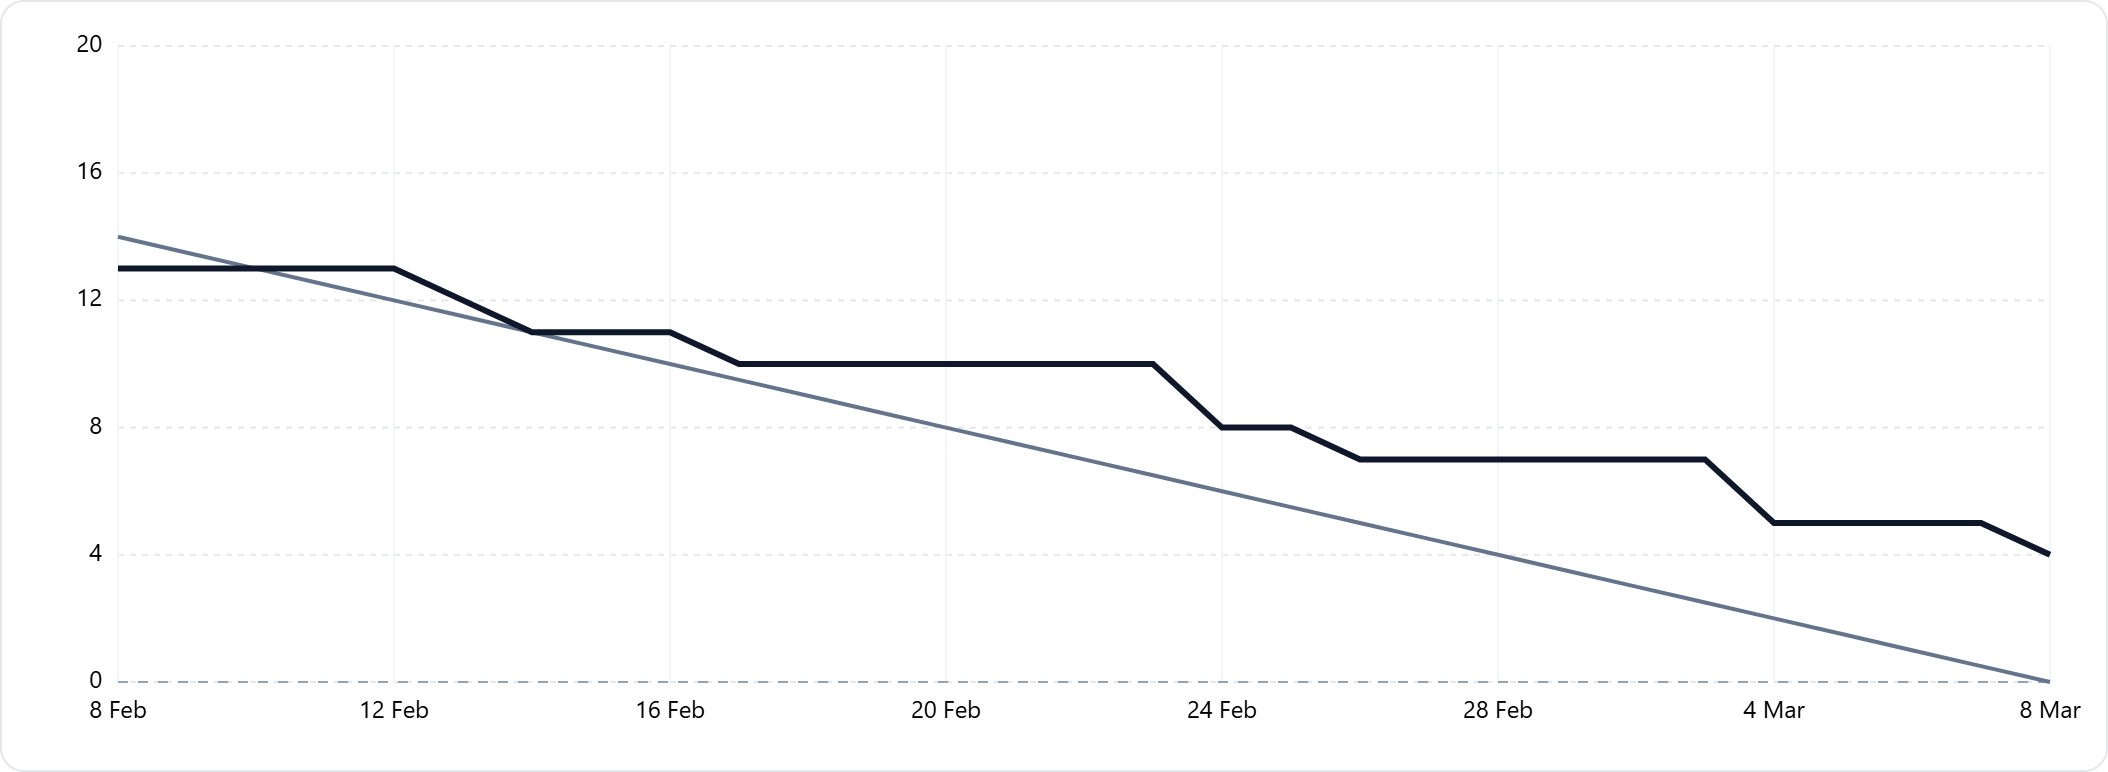
\includegraphics[width=\textwidth]{images/Sprint_1_-_Set-up_and_Basic_funcitonality-burndown.png}
    \caption{burndown chart of our first sprint}
    \label{fig:burndown-chart-sprint1}
\end{figure}

All tasks planned for the sprint were not finished:
Mainly sufficient testing for backend as well as set-up of database.
A lot of the delays in this period comes from difficulty with dealing with the large number of new frameworks to learn,
especially as a large amount of the work is dependent on the project being set-up, and so delays propagate.


\subsection{Sprint 2}

The timeframe for this sprint was the time between assignment 2 and 3.
08. March - 01. April

Goals:
The main goal of the second sprint is to make something that could ideally be presented to our target audience for evaluation and feedback.
There is therefore a large focus on the basic functionality required for a minimal viable product such as
functionality in our backend classes and database, an interactive frontend, as well as connection between frontend and backend.
Of course, related tasks such as presentations and reports are also included in the sprint.

\begin{figure}[H]
    \centering
    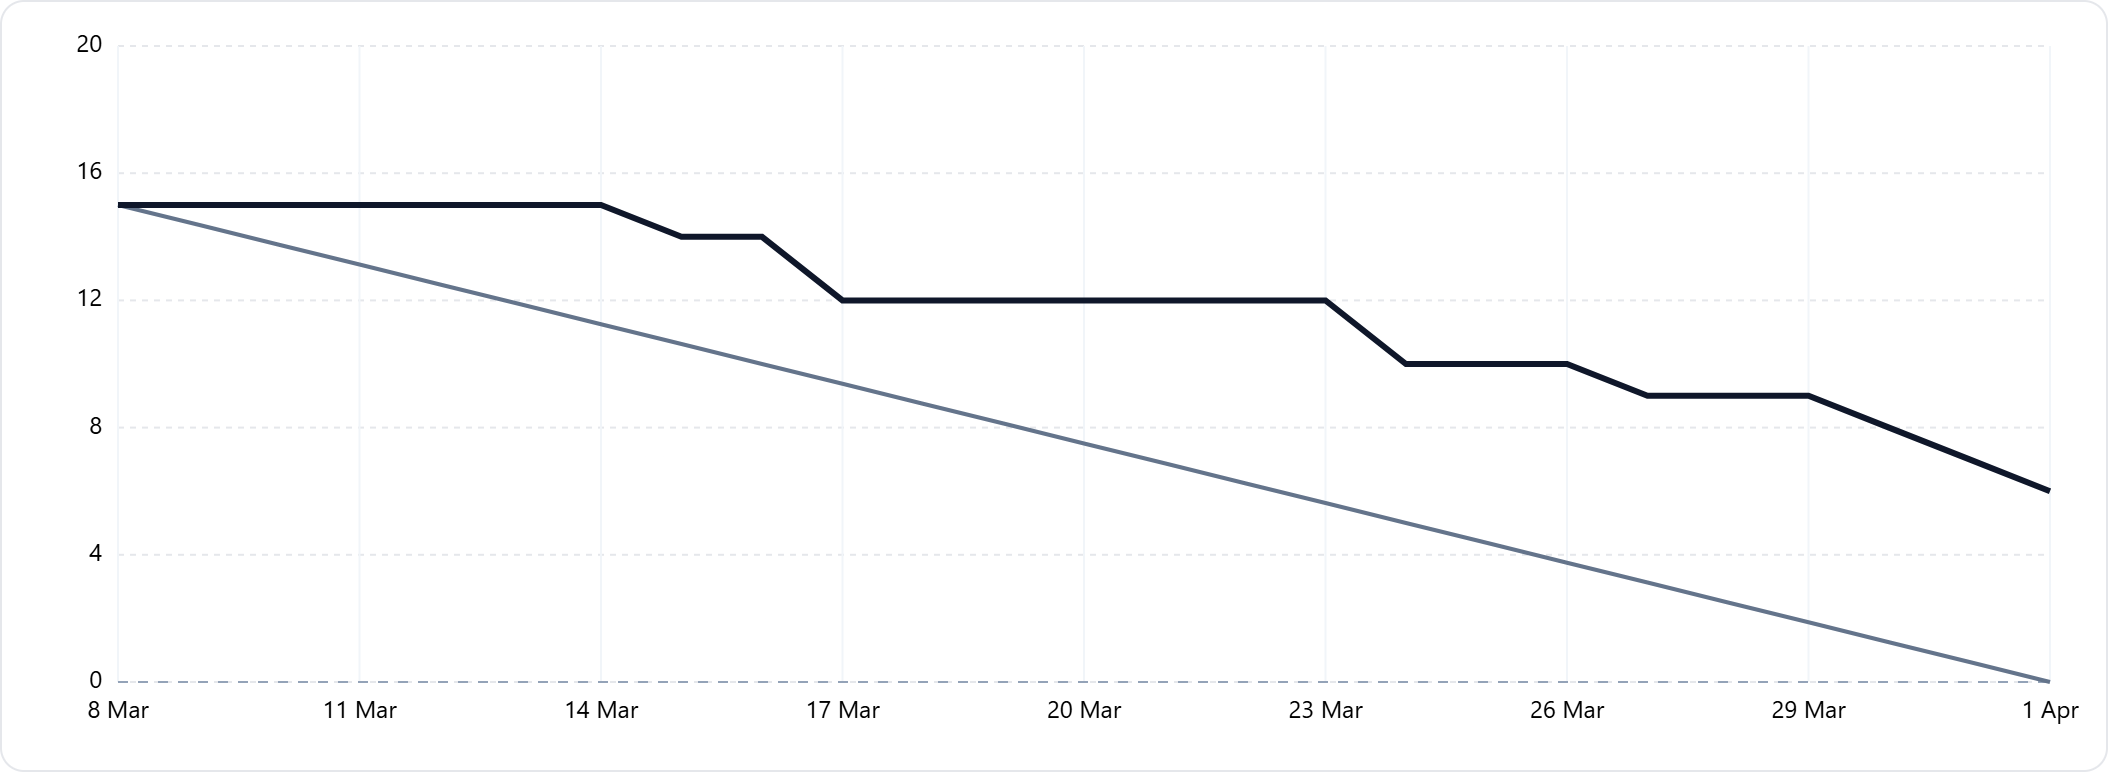
\includegraphics[width=\textwidth]{images/Sprint_2_-_Functionality_and_Refactoring-burndown}
    \caption{burndown chart of our second sprint}
    \label{fig:burndown-chart-sprint2}
\end{figure}


For backend, progress has been made in creating crud controllers for classes and setting up a persisting database.
For the front end, UI has improved significantly since the first iteration.
Again, the greatest challenge is that delays propagate.
Due to delays in important functional components such as the database,
as well as connection between frontend and backend, a lot of the work was backloaded to the
later parts of the sprint or not completed as scheduled.

\subsection{How Much Up-Front?}

Based on our experience in the project, we performed relatively little upfront architectural work.
This was mainly due to time constraints, learning new technologies, and a focus on delivering working functionality early in the development
This aligns with agile principles, where teams often aim to design “just enough” architecture to get started.

However, when reflecting on the paper, our approach may have been too far towards minimal upfront design.
The paper highlights that too little upfront planning can lead to an “accidental architecture”,
where decisions are made reactively rather than strategically.
While we have not yet encountered major issues caused by this,
there are clear areas where this could become problematic in later stages of the project.

For example, decisions regarding authentication and integration with external systems, such as using an existing student login solution,
have not been planned in advance.
Introducing such functionality later may require significant changes to both frontend and backend structure, indicating a potential architectural gap.

At the same time, our project included some factors such as needing to deliver functionality early, which supports a more emergent architecture approach.
According to the paper, this justifies reducing upfront work in order to remain flexible and responsive to change.

In hindsight, a slightly higher level of upfront architectural planning would likely have been beneficial,
especially in identifying external requirements and defining key system boundaries earlier.
This could have reduced the risk of future refactoring while still maintaining flexibility.

Overall, our architectural decisions were discussed, but not always systematically planned.
The project reflects the trade-off described in the paper.
Although our current approach has worked so far, a more balanced approach between upfront planning and emergent design would likely improve the system as it expands.
